\documentclass[sigconf]{acmart}
% defining the \BibTeX command - from Oren Patashnik's original BibTeX documentation.
\def\BibTeX{{\rm B\kern-.05em{\sc i\kern-.025em b}\kern-.08emT\kern-.1667em\lower.7ex\hbox{E}\kern-.125emX}}
% Remove the annoying stuff
\settopmatter{printacmref=false} % Removes citation information below abstract
\renewcommand\footnotetextcopyrightpermission[1]{} % removes footnote with conference information in first column
\pagestyle{plain} % removes running headers



\usepackage{Nikolai}




\begin{document}

%
% The "title" command has an optional parameter, allowing the author to define a "short title" to be used in page headers.
\title{CMIS Hand-in 1: Finite Difference Methods 1}

\author{Nikolai Plambech Nielsen}
\email{lpk331@alumni.ku.dk}
\affiliation{%
  \institution{Niels Bohr Institute, University of Copenhagen}
}


\maketitle

\section{Introduction}
When solving differential equations on a computer, one has several options. In this hand-in the finite difference method (FDM) is explored.

In general we are interested in calculating the evolution of a system with time over some domain, as it is governed by a partial differential equation. The domain is the ``space'' over which we solve the system, for example a line, surface or volume. We then sample this domain at a finite set of points, called the nodes of the system. All nodes then need to be updated for the system to evolve in time. The computational mesh is then the collection of all nodes in our domain.

For this hand in we are dealing with a regular mesh. This means that we sample the system at regular intervals in space, with a spacing of $ \Delta x $. An illustration of this can be seen in figure \ref{fig:reg_grid}.
\begin{figure}
	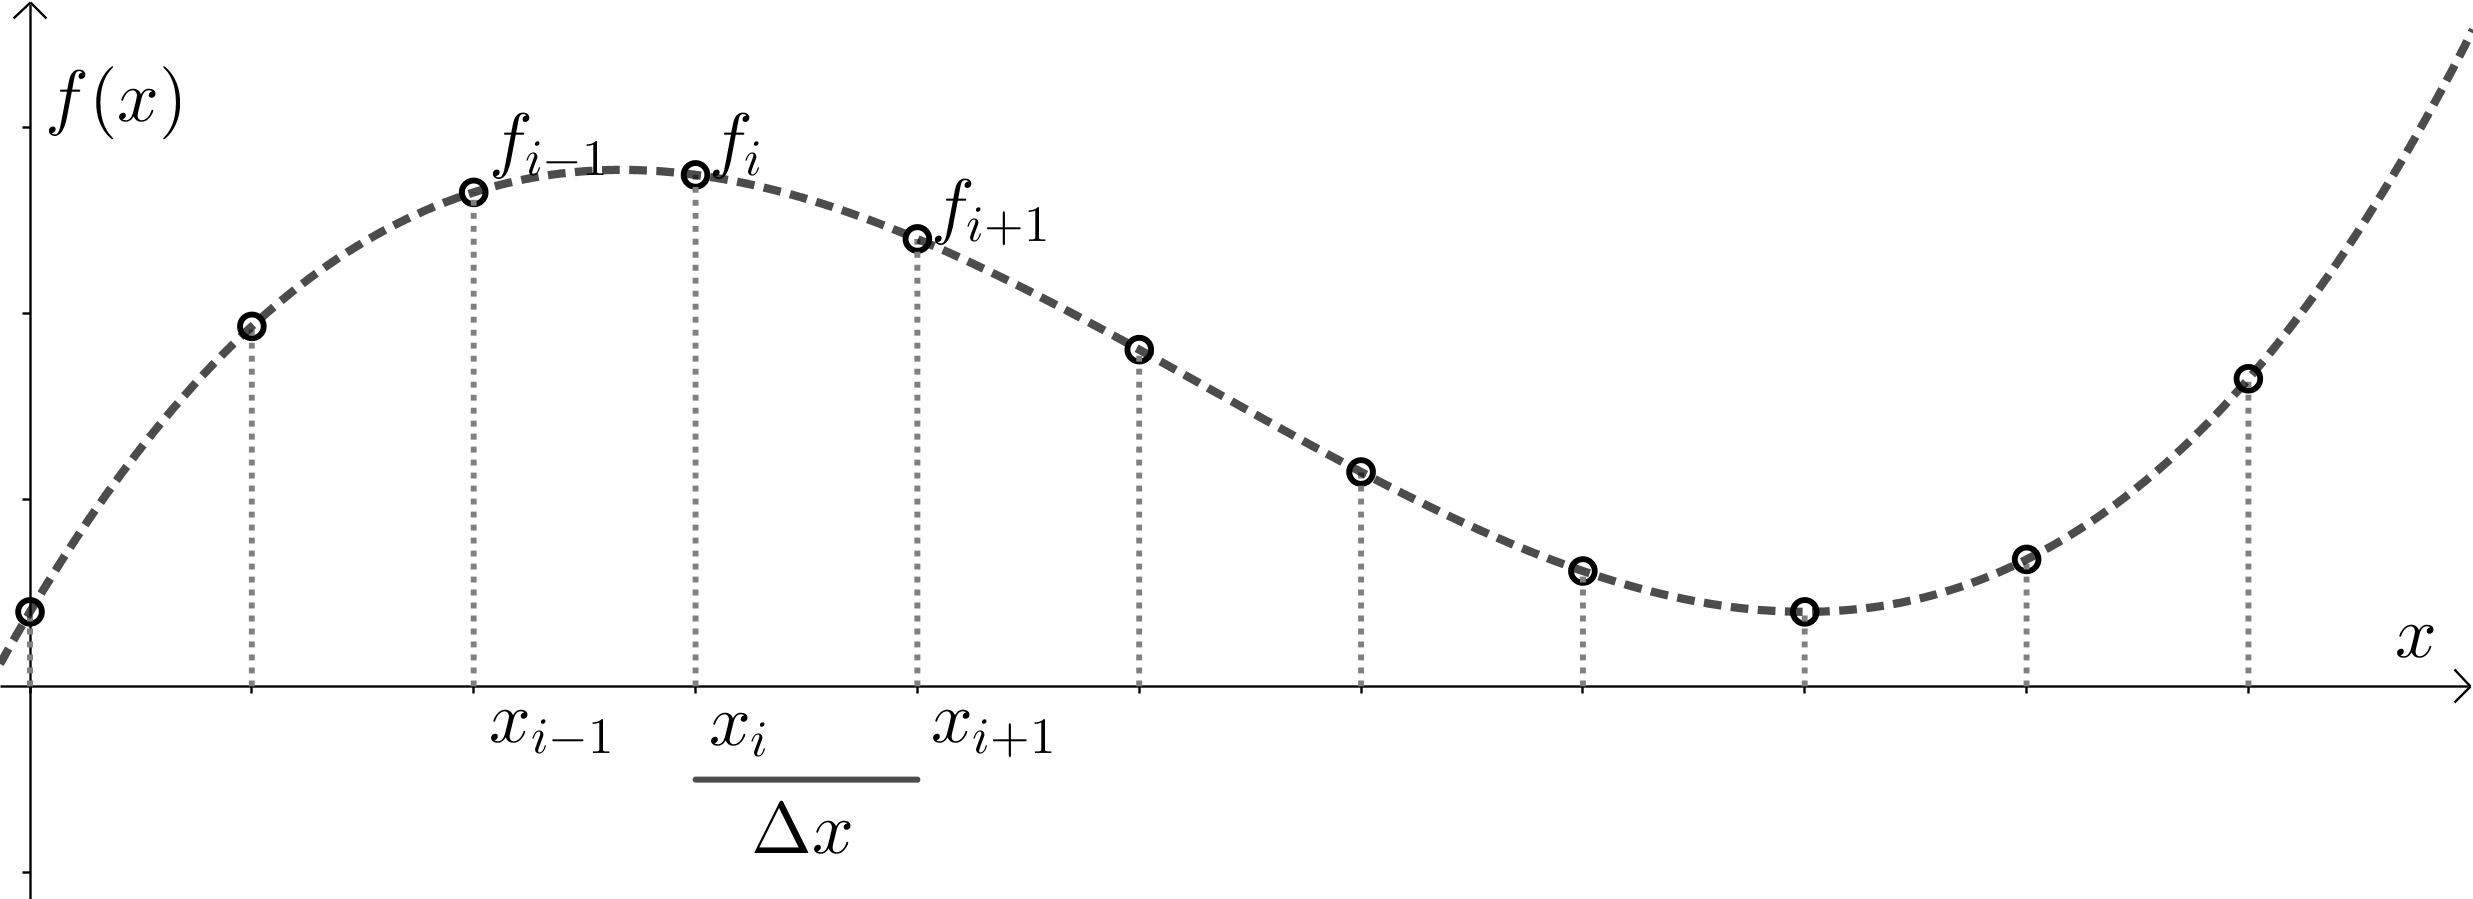
\includegraphics[width=\linewidth]{finite_difference1.png}
	\caption{A regular grid of nodes for some function $ f $}
	\label{fig:reg_grid}
\end{figure}

The $ x $-values are given by:
\begin{equation}\label{key}
	x_i = x' + i \Delta x
\end{equation}
where $ x' $ is usually taken as the origin, for convenience, and where $ i \in \{0,1,...,N\} $. The sampled values of the system $ f(x_i) $ are then denoted in shorthand by
\begin{equation}\label{key}
	f_i \equiv f(x_i)
\end{equation}
This of course generalises to higher dimensional systems. For two dimensions we have $ y_j = y' + j \Delta y$, and $ f_{i,j} \equiv f(x_i, y_j) $, and more indices for even higher dimensions.

\section{The Finite Difference Method}
The idea behind the finite difference method is to replace all derivatives in the equations with differences instead. This can be seen as not letting the spacing $ h $ in the differential quotient go all the way to zero, but just to some small value to get a reasonable approximation of it. Since we are working with regular grids, a convenient value is the spacing between points $ \Delta x $:
\begin{equation}\label{key}
	\diff[d]{f(x_i)}{x} = \lim\limits_{h\to 0} \frac{f(x_i + h) - f(x_i)}{(x_i+h) - x_i} \to \frac{f(x_i + \Delta x) - f(x_i)}{\Delta x}
\end{equation}
In this particular case, the finite difference is called the ``forward difference'' (FD) since it uses the point of interest $ x_i $ and the one next to it $ x_{i+1} = x_i + \Delta x $. In the compact notation we have
\begin{equation}\label{key}
	\diff[d]{f_i}{x} \approx \frac{f_{i+1} - f_{i}}{\Delta x}
\end{equation}
There is also the ``backwards difference'' (BD):
\begin{equation}\label{key}
	\diff[d]{f_i}{x} \approx \frac{f_{i} - f_{i-1}}{\Delta x}
\end{equation}
And the ``central difference'' (CD):
\begin{equation}\label{key}
	\diff[d]{f_i}{x} \approx \frac{f_{i+1} - f_{i-1}}{2 \Delta x}
\end{equation}
These can be shown explicitly from the Taylor Polynomials for $ f(x) $ around $ x_i $. There are of course also higher order differences. In particular we use the second order central difference when studying the heat equation, as this includes a second derivative:
\begin{equation}\label{key}
	\diff[d]{^2 f_i}{x^2} \approx \frac{f_{i-1} - 2f_i + f_{i+1}}{\Delta x^2}
\end{equation}
This, however, only takes care of calculating derivatives. What we want is to follow the evolution of the system with time. This means we have to do some sort of numerical time integration as well. But that is the subject of next weeks hand-in.

\subsection{Restrictions on parameters}
There are some considerations we need to make when designing the simulation of the system. In general we have some restrictions in the form of time, memory and accuracy.

These restrictions boil down to choosing the parameters of the system (for example $ \Delta x $ and $ \Delta y $ so as to get an acceptable trade-off between the restrictions).

The first concern is accuracy. We set out to solve some partial differential equation. This is all for naught, if we do not calculate an accurate result. The easiest way of increasing the accuracy is to decrease the spacing between the nodes. This of course results in more accurate approximations of the derivatives (with analytical results as $ \Delta x \to 0 $), but also increases both computation time and memory cost (if we keep the domain constant).

One might then think, given infinite time and memory - could we just keep decreasing the grid spacing $ \Delta x $ to get a more accurate result? It turns out we cannot, as the computer cannot resolve the difference between values accurately, as they approach each other.

To be more specific, the computer stores the numbers as floating points numbers, which in Numpy has a spacing of $ 2.2204 \D 10^{-16} $ (called the machine epsilon) for double precision floats (accessed by \texttt{numpy.finfo(float).eps}). Two numbers which differ by less than this value will be identical to the computer, and their difference will thus be 0. Trying to then divide by this difference (for example) will lead to crashing of the simulation.

\section{Constructing the simulation}
To construct a simulation, one discretises the governing equation, after which one has a couple of options. Either one can isolate the unknown $ u_{i,j} $, and loop over the computational mesh, updating each node in turn. Otherwise one can perform a matrix assembly of the system, where the discretised equation is expressed as a matrix equation to be solved, for example with a direct or iterative solver.  

In the discretisation step it can be useful to have a high-level overview of which values are needed to update each node. This is where the stencil comes in. This is is a schematic representation of which nodes are involved in each calculation. If, for example we want to calculate the second order derivative of a function at the point $ x_i $, using the second order centred difference, we will need the nodes $ x_i, x_{i+i} $ and $ x_{i-1} $. This can be graphically shown as in figure \ref{fig:stencil1}, where each node is represented by a circle. Usually we denote the unknown in the system by $ u $ and reserve $ f $ for known functions, called the source terms.
\begin{figure}
	\centering
	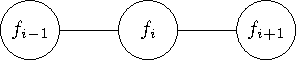
\includegraphics{stencil1.pdf}
	\caption{Stencil for the second order centred difference}
	\label{fig:stencil1}
\end{figure}



\section{Dealing with boundary conditions}
When on the boundary of the domain, ones options in discretisation is more limited. One cannot use the central difference, as there may be no node on one or the other side. Here we are presented with two major options: elimination of variables and using ghost notes. 

Elimination of variables makes use of forward/backwards differences at the borders, such that only existing nodes are used, while using ghost nodes means appending additional nodes to the borders of the domain, such that central differences can be used throughout the computational mesh.

\section{A Toy Problem}
In this toy problem we apply the concepts described above. We start with the 2D governing equation
\begin{equation}\label{key}
	(\nabla^2 - \kappa^2)u(x,y) = f(x,y),
\end{equation}
where $ \kappa > 0 $ and $ f $ is a known source term. Our domain is the unit square, with 4 samples in each direction, so $\Delta x = \Delta y = 1/3  $.

We apply the boundary conditions $ \partial u / \partial x = 0 $ on the vertical boundaries, and $ \partial u / \partial y $ on the horizontal boundaries. We further let $ f(x,y) = x+y $ and $ \kappa = 2 $. We handle the boundary conditions with ghost notes.

As such our computational mesh consists of 36 nodes, as shown in figure \ref{fig:matrix_assembly}, with the inner 16 nodes being the domain. In Python we start at the top left and then go down when looping over values of an array.
\begin{figure}
	\centering
	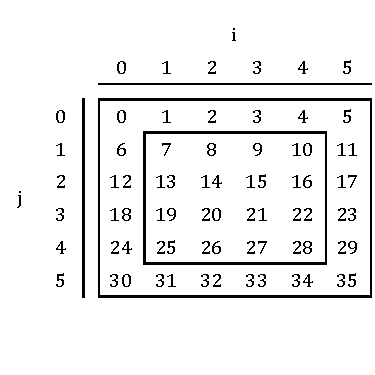
\includegraphics{indices.pdf}
	\caption{A graphic representation of the computational mesh.}
	\label{fig:matrix_assembly}
\end{figure}

The only term in the governing equation that needs discretisation is the laplacian, which we approximate as a sum of two central second order differences:
\begin{align}
	\nabla^2 u &= \diff{^2 u}{x^2} + \diff{^2 u}{y^2} \\
	&\approx \frac{u_{i+1, j} - 2 u_{i,j} + u_{i-1,j}}{\Delta x^2} + \frac{u_{i, j+1} - 2 u_{i,j} + u_{i,j-1}}{\Delta y^2}.
\end{align}
Collecting all the different terms we get
\begin{equation}\label{key}
	\sum_{k = -1}^{1} \sum_{k' = -1}^{1} c_{i+k, j+k'} u_{i+k, j+k'} = f_{i,j}
\end{equation}
with
\begin{align}\label{key}
	c_{i-1,j} &= c_{i+1, j} = \Delta x^{-2} \\
	c_{i,j-1} &= c_{i, j+1} = \Delta y^{-2} \\
	c_{i,j} &= -\kappa^2 - 2\Delta x^{-2} - 2\Delta y^{-2}
\end{align}
for a stencil as seen in figure \ref{fig:stencil2}
\begin{figure}
	\centering
	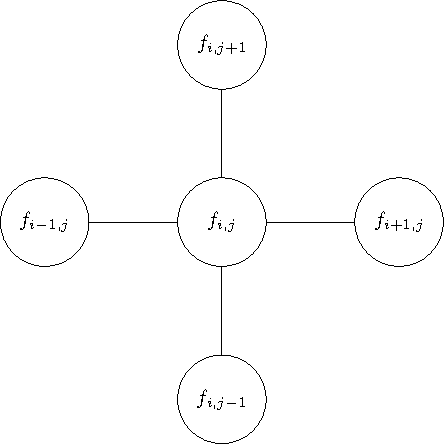
\includegraphics{stencil.pdf}
	\caption{Stencil for the toy problem}
	\label{fig:stencil2}
\end{figure}

\subsection{Updating formulas}
From here it is easy to isolate $ u_{i,j} $ to get the update formula for the domain nodes:
\begin{equation}\label{key}
	u_{i,j}  = \frac{1}{c_{i,j}} \pp{f_{i,j} - \sum_{k = -1, 1}\sum_{k' = -1, 1} c_{i+k, j+k'} u_{i+k, j+k'}}
\end{equation}
For the boundary condition we need the first derivative on the boundary to be zero. Using a central difference on the left border we get
\begin{equation}\label{key}
\diff{u_{1,j}}{x} =\frac{u_{2,j} - u_{0,j}}{2\Delta x} = 0 \Rightarrow u_{0,j} = u_{2,j},
\end{equation}
and similarly for the other boundaries, giving us the updating formula for the boundary nodes. To update the computational mesh we first update the ghost notes, and after that the domain nodes using the above updating formulas.

\subsection{Matrix Assembly}
For the matrix assembly we stack up all the nodes in the 2D computational mesh $ u $ into a single 1D column vector, with the order given in figure \ref{fig:matrix_assembly}. This is exactly the way \texttt{np.flatten} works. If we label the vector by $ n $, then $ n = N_y i + j $, where $ N_y $ is the number of nodes in the $ y $ direction. The coefficients for each node can then be written up in a row of an $ N_xN_y \times N_x N_y $ matrix $ A $. The source term $ f $ is of course flattened in a similar way to the vector $ u $.

Take the node $ i=2, j=3 $, as an example. This node is in the domain, with $ n=6\D2+3 = 15 $. This then corresponds to the 16th row of $ A $. Looking at the stencil we see that 5 entries of the row are populated, $ m \in \{9, 14, 15, 16, 21\} $.

For the ghost nodes to follow the boundary conditions we need $ c_{0,j} = - c_{2,j} $ and $ f_{0,j}=0 $ for the matrix equation to hold (or similarly for the top/right/bottom border). This then ensures that the derivative at $ i=1, j $ is zero (in the central difference approximation).

With these two specifications, 32 rows of the matrix have been specified. However, the rows corresponding to the corner ghost nodes have yet to be filled in. If they are not, then the matrix will be singular due to these rows of zeros and a direct solver like \texttt{np.linalg.solve} cannot be used. Since no other nodes use the values of the corner ghost nodes, we just set $ c_{i,j} = 1 $ for each of the corner nodes. Spying on this matrix we see the following (figure \ref{fig:spy})
\begin{figure}
	\centering
	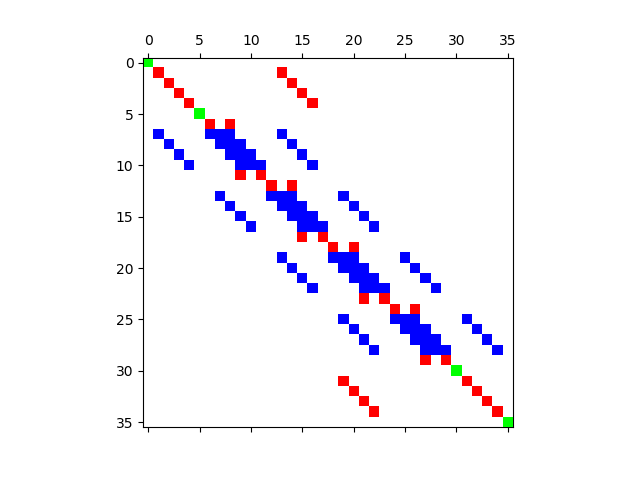
\includegraphics[width=\linewidth]{spy.png}
	\caption{Spying on the matrix $ A $. Rows with green correspond to corner ghost nodes. Red to regular ghost nodes and blue to nodes in the domain.}
	\label{fig:spy}
\end{figure}
And indeed, we have four rows of domain nodes, each with 5 elements filled in, separated by two side-ghost nodes (which can be seen since there is an empty element between the 2 filled in). At the ``ends'' we have a corner, 4 ghost nodes and another corner.

With the matrix assembled the system $ Au=f $ can be solved to get the next step.

\subsection{Results}
\begin{figure}
	\centering
	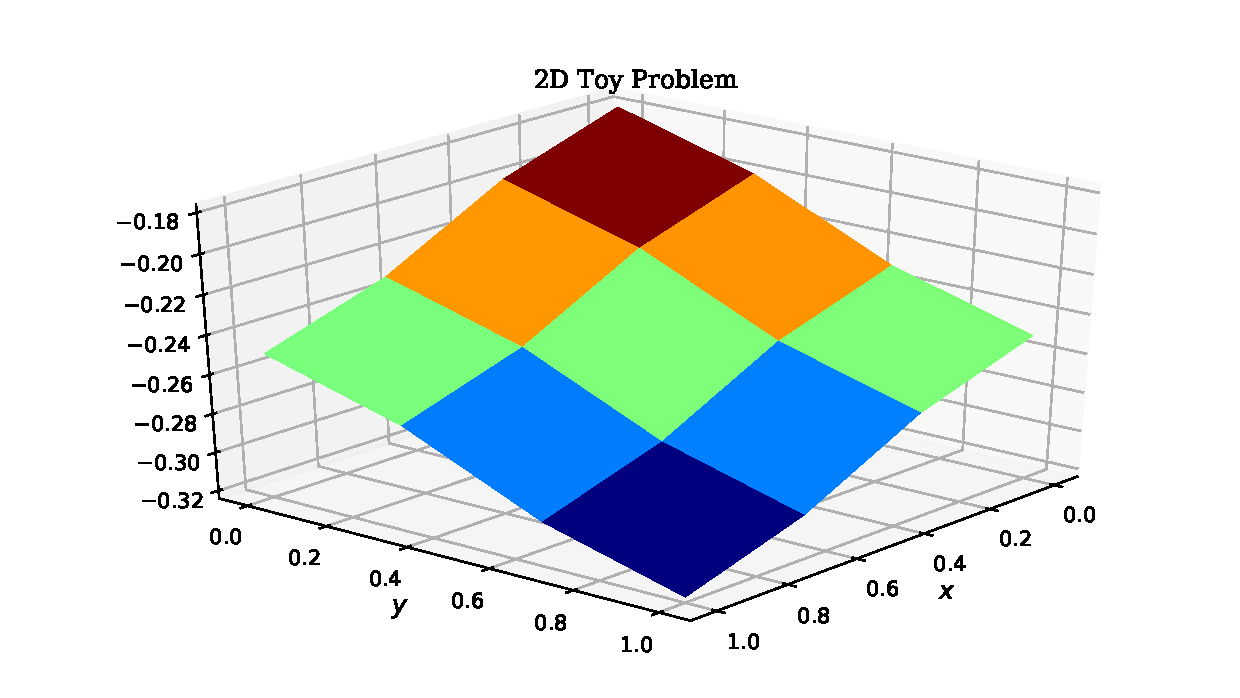
\includegraphics[width=\linewidth]{result1.pdf}
	\caption{result from the toy problem, with $ n=4 $}
	\label{fig:result1}
\end{figure}
After the equation has been solved, the result $ u $ has to be reassembled into a 2D array for plotting. This is done with the \texttt{np.reshape} command. With $ u $ back in the proper shape, we can plot the result (without the ghost nodes, of course). These are shown in figures \ref{fig:result1}, \ref{fig:result2} and \ref{fig:result3} with $ n=4,10,100 $ respectively.

\begin{figure}
	\centering
	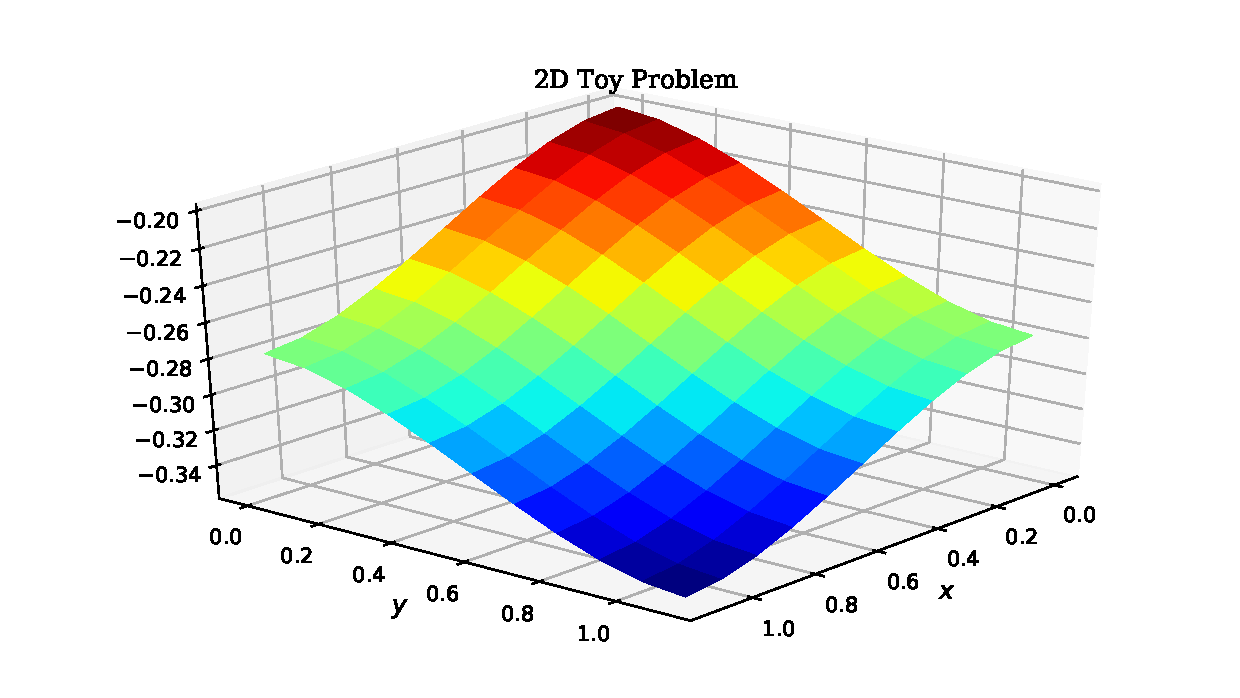
\includegraphics[width=\linewidth]{result2.pdf}
	\caption{result from the toy problem, with $ n=10 $}
	\label{fig:result2}
\end{figure}

\begin{figure}
	\centering
	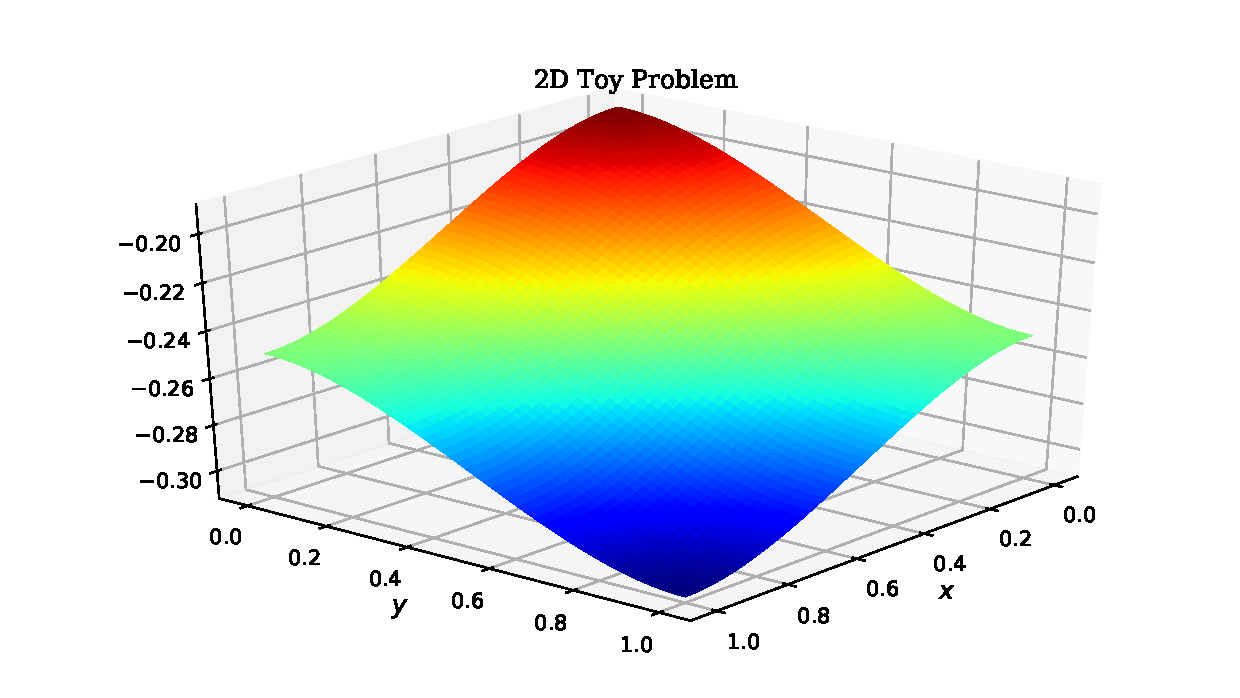
\includegraphics[width=\linewidth]{result3.pdf}
	\caption{result from the toy problem, with $ n=100 $}
	\label{fig:result3}
\end{figure}

Our intuition says that the result should not depend highly on $ n $ (except in the pathological cases of $ n = 1 $ where our approximations break down, and $ n \to \infty $ where numerical blow up will happen). To make this clear, the maximum and minimum value of $ u $ are tabulated in table \ref{tab:min_max} (the max and min happen at (0,0) and (1,1) respectively):
\begin{table}
	\centering
	\begin{tabular}{ccc}
		\hline
		$ n $ & min & max \\
		\hline
		4 & -0.321 & -0.179 \\
		10 & -0.356 & -0.200 \\
		100 & -0.310 & -0.190 \\
		150 & -0.312 & -0.191 \\
		\hline 
	\end{tabular}
	\caption{Table of minimum and maximum values of $ u $}
	\label{tab:min_max}
\end{table}
This measure of the accuracy of the simulation might not be the best, but it is at least in the same order of magnitude for all $ n $ calculated.


\section{A second toy problem}
In the second toy problem we look at the governing equation
\begin{equation}\label{key}
	\diff{^2 u}{x^2} = 0
\end{equation}
on the domain $ x \in [0,1] $, with boundary conditions $ du/dx=0 $ at both edges, realised by ghost nodes, and $ n>3 $.

For this problem we again use a second order central difference for the discretisation, resulting in the stencil seen in figure \ref{fig:stencil1}. The matrix assembly is considerably easier as $ u $ is already a column vector.

For the boundary condition we use the central difference giving $ c_0=c_{n+1}=(2\Delta x)\inverse $ and $ c_2=c_{n-1}= -(2\Delta x)\inverse $, with $ f_0 = f_{n+1} = 0 $. Spying on the matrix $ A $ gives the picture seen in figure \ref{fig:spy_2}
\begin{figure}
	\centering
	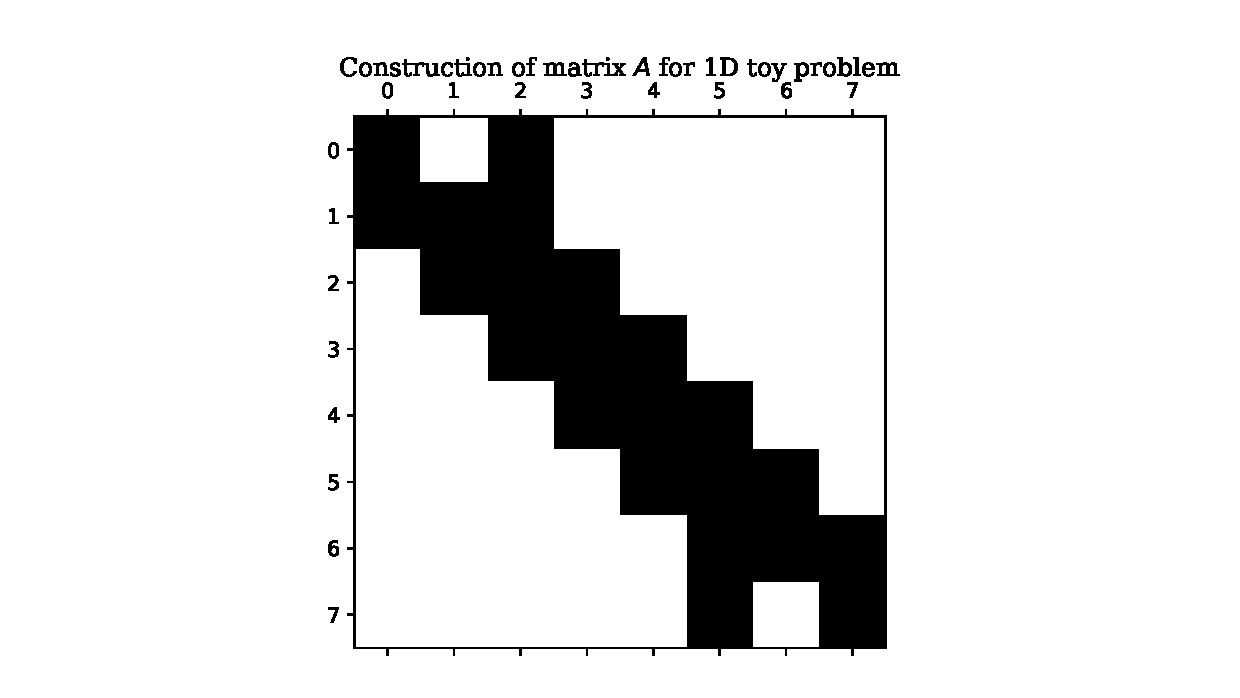
\includegraphics[width=\linewidth]{spy_2.pdf}
	\caption{Structure of the matrix $ A $ for the 1D toy problem. $ n=6 $}
	\label{fig:spy_2}
\end{figure}
This matrix has rank 7 (and size 8), with eigenvalues tabulated in the first column of table \ref{tab:eigs}. As seen, the seventh eigenvalue is of the order $ \epsilon $, and is therefore most likely 0. This is to be expected for a matrix with rank $ n-1 $.
\begin{table}
	\centering
	\begin{tabular}{cc}
		\hline
		2 derivative BCs & 1 derivative BC \\
		\hline
		-94.917   & -94.998    \\
		-80.825    & -81.055     \\
		-60.863   & -61.104   \\
		-39.296   &-39.258   \\
		-20.394   & -19.854   \\
		-7.379    & -6.453    \\
		$ 1.938  \D 10^{-16} $& -0.616\\
		-1.326 & 0.838 \\
		\hline
	\end{tabular}
	\caption{Table of eigenvalues for the matrix $ A $ with different boundary conditions}
	\label{tab:eigs}
\end{table}
The clue to construct a matrix for the system with full rank lies in analysing the governing equation. Integration twice gives
\begin{equation}\label{key}
	\iint \diff{^2 u}{x^2} dx = u = \diff{u}{x} x + a
\end{equation}
which is just a straight line. To fully specify the solution we need the derivative of the line, and some fixed point (like the intersection with the $ u $-axis). Our boundary conditions gives us the derivative, but an intersection is still missing. Incorporating a different boundary condition on one side (say $ u_b = b $) would provide a fixed point, the specific solution, a full rank matrix and 8 non-zero eigenvalues.

As an example we set $ u_b = 1 $ for the ghost node, corresponding to $ c_n = 1 $ and $ f_{n+1} = 1 $ for the ghost node row. The eigenvalues are tabulated in the second column of table \ref{tab:eigs}. The result of this simulation is seen in figure \ref{fig:1d_result.pdf}, and sure enough $ u = 1 $ for all $ x $.
\begin{figure}
	\centering
	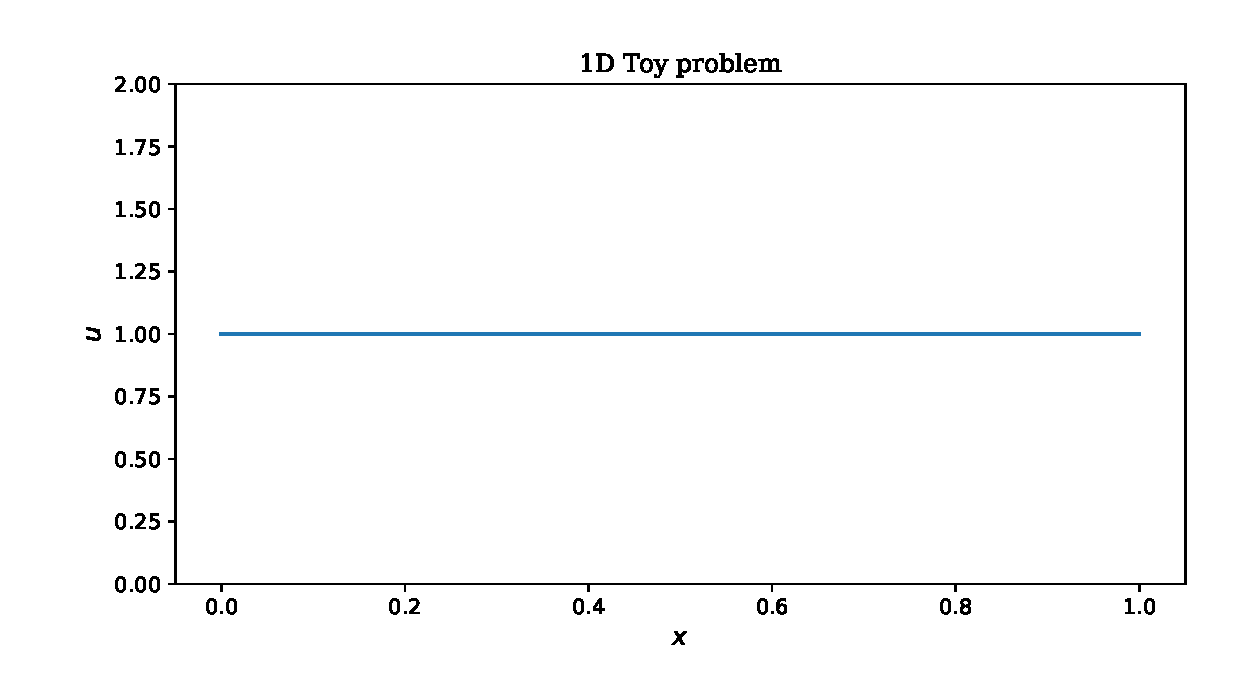
\includegraphics[width=\linewidth]{1d_result.pdf}
	\caption{The 1D toy example, with a full rank matrix $ A $.}
	\label{fig:1d_result.pdf}
\end{figure}


 



\end{document}
